\documentclass{beamer} % [aspectratio=169]
\usetheme{ucl}
\setbeamercolor{banner}{bg=darkred}
\setbeamersize{description width=2em}
\setbeamertemplate{navigation symbols}{\vspace{-2ex}} 

%\usepackage{fontspec}
\usepackage[utf8]{inputenc}
% \usepackage[english, greek]{babel}


\usepackage[T1]{fontenc} % Turn £ into $
\usepackage{minted}
\usemintedstyle{emacs}

\usepackage{fancyvrb}
\usepackage{xcolor}
\usepackage{url}

\usepackage{natbib}
\usepackage{bibentry}
\usepackage{url}


\usepackage{tikz}
\usetikzlibrary{positioning}


\newcommand\emc[1]{\textcolor{midred}{\textbf{#1}}}

\AtBeginSection[]{
  \begin{frame}
  \vfill
  \centering
  \begin{beamercolorbox}[sep=8pt,center,shadow=true,rounded=true]{title}
    \usebeamerfont{title}\insertsectionhead\par%
  \end{beamercolorbox}
  \vfill
  \end{frame}
}

\author{Prof.\ Mark Handley, University College London, UK}
\title{Dynamic Data Structures and Algorithms.}
\subtitle{ENGF0002: Design and Professional Skills }
% \institute{}
\date{Term 1, 2018}


\begin{document}
\nobibliography*


\frame{
\titlepage
}

\begin{frame}
  \centering
  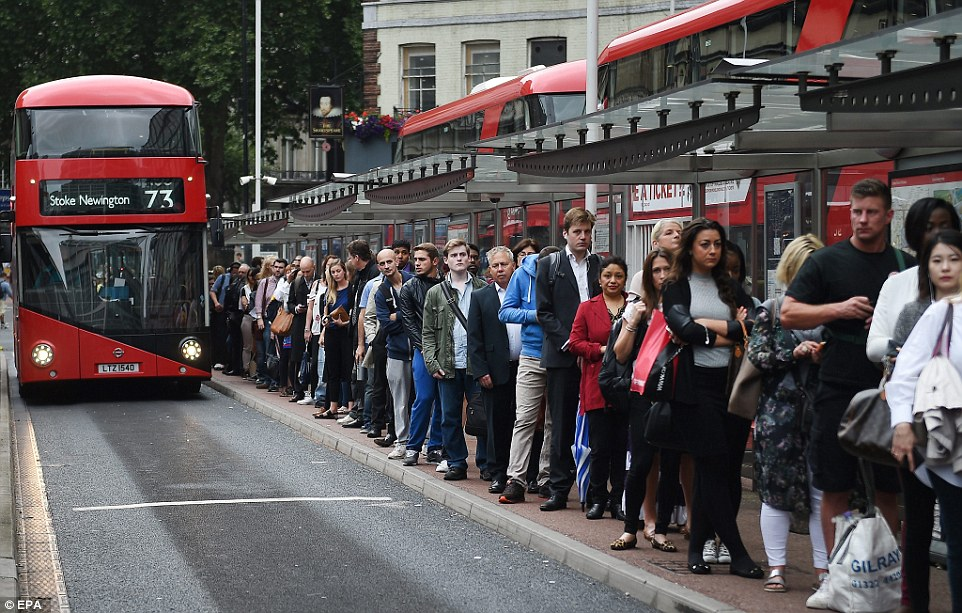
\includegraphics[width=70mm]{assets/bus-queue.jpg}
\end{frame}

\begin{frame}
\frametitle{Today's topics}

\begin{itemize}
\item Understand how dynamic data types are implemented.
\item Explore in detail how to implement linked lists.
\item Introduce Object Oriented Programming
\item Implement a data type that maintains a sorted set of data using a tree.
\end{itemize}

\end{frame}

\begin{frame}
\frametitle{A Node class for a linked list.}

	\inputminted[
		firstline=1,
		lastline=4,
		xleftmargin=1.4em,
		%frame=lines,
		%framesep=2mm,
		fontsize=\footnotesize,
                bgcolor=stone,
		linenos
	]{python}{src/linked_list.py}

        A class defines a new data type.
        \begin{itemize}
        \item It can contain data.
        \item It can contain functions that act on that data
        \end{itemize}
\end{frame}

\begin{frame}
\frametitle{A Node class for a linked list.}

	\inputminted[
		firstline=1,
		lastline=4,
		xleftmargin=1.4em,
		%frame=lines,
		%framesep=2mm,
		fontsize=\footnotesize,
                bgcolor=stone,
		linenos
	]{python}{src/linked_list.py}

        The \texttt{\_\_init\_\_()} function is special.  It is called when a new instance of the class is created.
	\inputminted[
		firstline=68,
		lastline=68,
		xleftmargin=1.4em,
		%frame=lines,
		%framesep=2mm,
		fontsize=\footnotesize,
                bgcolor=stone,
		linenos
	]{python}{src/linked_list.py}

\end{frame}

\begin{frame}
\frametitle{Helper functions make the API more obvious}

	\inputminted[
		firstline=1,
		lastline=10,
		xleftmargin=1.4em,
		%frame=lines,
		%framesep=2mm,
		fontsize=\footnotesize,
                bgcolor=stone,
		linenos
	]{python}{src/linked_list.py}

        A test for node initialization:
	\inputminted[
		firstline=68,
		lastline=70,
		xleftmargin=1.4em,
		%frame=lines,
		%framesep=2mm,
		fontsize=\footnotesize,
                bgcolor=stone,
		linenos
	]{python}{src/linked_list.py}

\end{frame}

\begin{frame}
\frametitle{Adding to a linked list is fast}

	\inputminted[
		firstline=1,
		lastline=4,
		xleftmargin=1.4em,
		%frame=lines,
		%framesep=2mm,
		fontsize=\footnotesize,
                bgcolor=stone,
		linenos
	]{python}{src/linked_list.py}

        Appending to an existing node just requires updating the \texttt{next} node field.
	\inputminted[
		firstline=12,
		lastline=15,
		xleftmargin=1.4em,
		%frame=lines,
		%framesep=2mm,
		fontsize=\footnotesize,
                bgcolor=stone,
		linenos
	]{python}{src/linked_list.py}
\end{frame}

\begin{frame}
\frametitle{Adding anywhere in a linked list is fast}

	\inputminted[
		firstline=1,
		lastline=4,
		xleftmargin=1.4em,
		%frame=lines,
		%framesep=2mm,
		fontsize=\footnotesize,
                bgcolor=stone,
		linenos
	]{python}{src/linked_list.py}
        \vspace{-5mm}
	\inputminted[
		firstline=30,
		lastline=34,
		xleftmargin=1.4em,
		%frame=lines,
		%framesep=2mm,
		fontsize=\footnotesize,
                bgcolor=stone,
		linenos
	]{python}{src/linked_list.py}
        \vspace{-5mm}
	\inputminted[
		firstline=116,
		lastline=122,
		xleftmargin=1.4em,
		%frame=lines,
		%framesep=2mm,
		fontsize=\footnotesize,
                bgcolor=stone,
		linenos
	]{python}{src/linked_list.py}
        
\end{frame}

\begin{frame}
\frametitle{Deletion anywhere in a linked list is fast}

	\inputminted[
		firstline=1,
		lastline=4,
		xleftmargin=1.4em,
		%frame=lines,
		%framesep=2mm,
		fontsize=\footnotesize,
                bgcolor=stone,
		linenos
	]{python}{src/linked_list.py}
        \vspace{-5mm}
	\inputminted[
		firstline=26,
		lastline=28,
		xleftmargin=1.4em,
		%frame=lines,
		%framesep=2mm,
		fontsize=\footnotesize,
                bgcolor=stone,
		linenos
	]{python}{src/linked_list.py}
        \vspace{-5mm}
	\inputminted[
		firstline=122,
		lastline=124,
		xleftmargin=1.4em,
		%frame=lines,
		%framesep=2mm,
		fontsize=\footnotesize,
                bgcolor=stone,
		linenos
	]{python}{src/linked_list.py}
        
\end{frame}

\begin{frame}
\frametitle{Indexing into a linked list requires O(n) time}

	\inputminted[
		firstline=1,
		lastline=4,
		xleftmargin=1.4em,
		%frame=lines,
		%framesep=2mm,
		fontsize=\footnotesize,
                bgcolor=stone,
		linenos
	]{python}{src/linked_list.py}
        \vspace{-5mm}
	\inputminted[
		firstline=51,
		lastline=56,
		xleftmargin=1.4em,
		%frame=lines,
		%framesep=2mm,
		fontsize=\footnotesize,
                bgcolor=stone,
		linenos
	]{python}{src/linked_list.py}
        \vspace{-5mm}
	\inputminted[
		firstline=124,
		lastline=127,
		xleftmargin=1.4em,
		%frame=lines,
		%framesep=2mm,
		fontsize=\footnotesize,
                bgcolor=stone,
		linenos
	]{python}{src/linked_list.py}
        
\end{frame}


\section{Visualization Diversion}

\section{Bomber Programme}

\begin{frame}
  \frametitle{Bug 1:  Bomb doesn't come back when it misses buildings}
  \textbf{Cause of bug:}  missing test for bomb hitting ground.
	\inputminted[
		firstline=235,
		lastline=242,
		xleftmargin=1.4em,
		%frame=lines,
		%framesep=2mm,
		fontsize=\footnotesize,
                bgcolor=stone,
		linenos
	]{python}{assets/bomber_oo.py}

  Missing tests are common causes of bugs in code.  This one is pretty obvious, but they're often not obvious, and only hit very rarely.  Big source of obscure runtime errors.
\end{frame}

\begin{frame}
  \frametitle{Bug 2:  Can't bomb right hand building}
  \textbf{Cause of bug:}  plane doesn't wrap far enough right.  Wrong constant used to move the plane.

	\inputminted[
		firstline=168,
		lastline=172,
		xleftmargin=1.4em,
		%frame=lines,
		%framesep=2mm,
		fontsize=\footnotesize,
                bgcolor=stone,
		linenos
	]{python}{assets/bomber_oo.py}

\textbf{Fix:} move the plane by \texttt{CANVAS\_WIDTH + self.width}.
\end{frame}

\begin{frame}
  \frametitle{Bug 3:  Too many buildings}
  
  \textbf{Symptom}: If you fix Bug 2, the plane hits a building off the right side of the screen.
  \textbf{Cause}:  magic embedded constant is wrong

	\inputminted[
		firstline=219,
		lastline=229,
		xleftmargin=1.4em,
		%frame=lines,
		%framesep=2mm,
		fontsize=\footnotesize,
                bgcolor=stone,
		linenos
	]{python}{assets/bomber_oo.py}
        
        \vspace{-5mm}\textbf{Fix:} replace \texttt{1200} with \texttt{CANVAS\_WIDTH}
        
        \textbf{Lesson:} don't embed random magic numbers - try to use named constants
\end{frame}

\begin{frame}
  \frametitle{Bug 4:  Plane can't land}
  
  \textbf{Cause}:  test preventing going off the bottom of screen is wrong due to bad assumptions about what the plane position represents.

	\inputminted[
		firstline=172,
		lastline=175,
		xleftmargin=1.4em,
		%frame=lines,
		%framesep=2mm,
		fontsize=\footnotesize,
                bgcolor=stone,
		linenos
	]{python}{assets/bomber_oo.py}
        
        \textbf{Fix:} \texttt{Plane.position.getY()} returns the top of the plane.  Test should test the bottom of the plane.  
\end{frame}

\begin{frame}
  \frametitle{Bug 5:  Bomb scrapes the left side of a building without exploding}
  \centering
  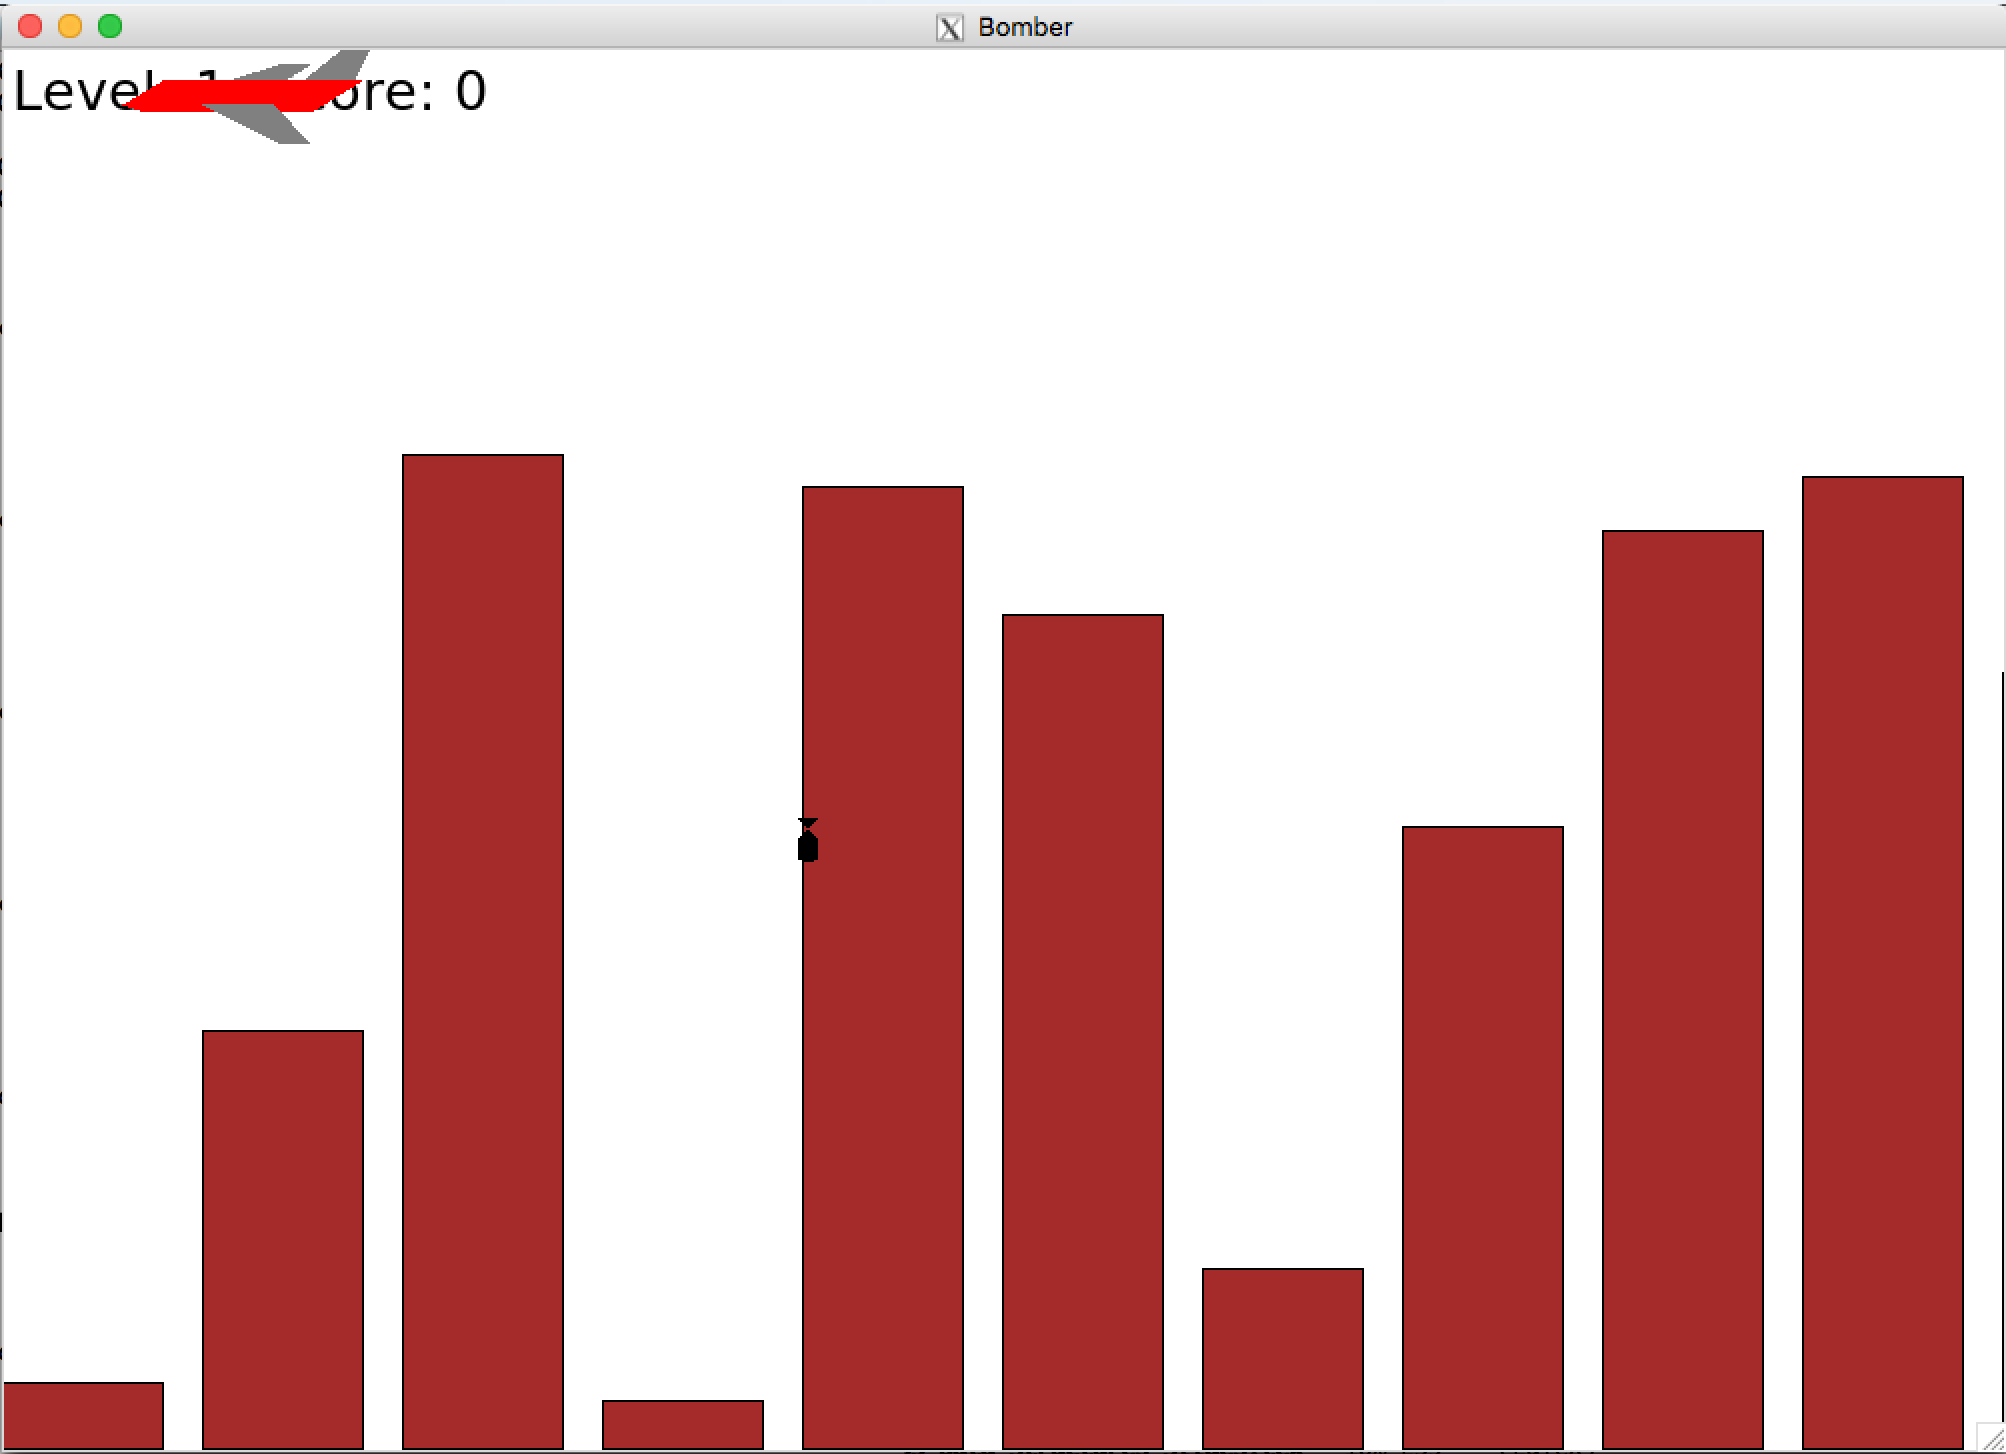
\includegraphics[width=90mm]{assets/bomb-scrape.png}
\end{frame}

\begin{frame}
  \frametitle{Bug 5:  Bomb scrapes the left side of a building without exploding}
  
  \textbf{Cause}:  test only tests whether top left corner of bomb is inside a building.

	\inputminted[
		firstline=238,
		lastline=242,
		xleftmargin=1.4em,
		%frame=lines,
		%framesep=2mm,
		fontsize=\footnotesize,
                bgcolor=stone,
		linenos
	]{python}{assets/bomber_oo.py}
        
        \textbf{Fix:} also test if the top right corner of the bomb is in a building
\end{frame}


\bibliographystyle{alpha}
\nobibliography{references}

\end{document}
